\subsection{Data Collection from Simulation}

To test Fido's effectiveness at learning with limited feedback, Fido was first trained on a number of different tasks through our simulator using reward values delegated through software.
Data was collected regarding Fido's latency and number of reward iterations needed for convergence.

\subsubsection{Simulation Experiments}

Fido's first and simplest task, dubbed ``Flash,'' was to set the brightness value of an LED to a value proportional to the amount of light that Fido sensed.
Each reward iteration, Fido's neural network was given the intensity of visible light that Fido detected and was asked for the brightness value of Fido's LED.
Fido was then given a reward value equal to $1 - |b - v|$ where $b$ was the brightness value of Fido's LED ranging from 0 to 1 and $v$ was the intensity of visible light that Fido detected ranging from 0 to 1.
Fido's feed-forward neural network had 3 hidden layers each with 10 neurons and outputted 4 wires to the wire-fitted interpolator.
As for all of the tasks, Fido's neural network's input and hidden layers used a sigmoid activation function, while  its output layer used a linear activation function that simply outputted its input.
The exploration constant in equation \ref{equ::boltzmann} was held at 0.2 for the duration of the task.

``Float,'' Fido's second task, challenged our learning implementation to direct a robot to point.
Each time it was told to select an action, Fido specified the robot's vertical and horizontal velocity between +10 and -10 pixels.
This emulates a holonomic drive systems, where motor outputs directly correlate to movement on the $x$ and $y$ axes.
At the start of each trial, Fido and the point were placed randomly on a boundless plane within 768 pixels of one another.
Fido was fed the ratio of its $x$ displacement to its $y$ displacement from its target point as the state.
Every fourth action that Fido made was chosen as a reward iteration, and Fido was given a reward value corresponding to its last action.
This reward value was the difference between Fido's distance away from the target point before performing the action and Fido's distance from the target point after performing the action.
Fido completed each trial when it was within 70 pixels of the point.
Fido's feed-forward neural network had 3 hidden layers each with 10 neurons and outputted 3 wires to the wire-fitted interpolator.
The exploration constant in equation \ref{equ::boltzmann} was held at 0.15.

Fido's next task, nicknamed ``Drive,'' required that it direct a robot to point by controlling the motors of a differential drive system.
At the start of each trial, Fido and the point were placed randomly on a boundless plane within 768 pixels of one another.
Fido was fed the ratio of its $x$ displacement to its $y$ displacement from its target point as well as its rotation.
Every fourth action that Fido made was chosen as a reward iteration, and Fido was given a reward value corresponding to its last action.
This reward value was the difference between Fido's distance away from the target point before performing the action and Fido's distance from the target point after performing the action.
Fido completed each trial when it was within 70 pixels of the point.
Fido's feed-forward neural network had 4 hidden layers each with 10 neurons and outputted 5 wires to the wire-fitted interpolator.
The exploration constant in equation \ref{equ::boltzmann} was held at 0.2.

Fido's last challenge, called ``Follow,'' was to perform the classic robotic task of line following by controlling the motors of the simulator's differential drive system.
At the start of each trial, Fido and a line with a random rotation were placed arbitrarily on a boundless plane within 768 pixels of one another.
Fido was fed the ratio of its $x$ displacement to its $y$ displacement from the closest point on the line as well as its rotation.
Every second action that Fido made was chosen as a reward iteration.
An action's reward value was the difference between Fido's distance away from the line before performing the action and Fido's distance from the line after performing the action.
Fido completed each trial when it had stayed within 60 pixels of the line for 10 consecutive actions (5 reward iterations).
Fido's feed-forward neural network had 4 hidden layers each with 10 neurons and outputted 4 wires to the wire-fitted interpolator.
The exploration constant in equation \ref{equ::boltzmann} was held at 0.2.

\subsubsection{Simulation Findings}

Each task was run 500 times to gather the data show in Table \ref{tab:data}.
 The reward iterations values shown in the above data table were the medians of the data collected.
The median is shown instead of the mean to discount a few large outliers that were present in data.
The time data shown above is the mean of the data collected.

\begin{table}[ht]
	\centering
	\begin{tabular}{@{}lccc@{}}
		\toprule
		Task        & Learning Iterations & Action Selection (ms) & Training Time (ms) \\ \midrule
		Flash       & 6                   & 0.
                 & 6               \\
		Float       & 14                  & 1                  & 6               \\
		Drive       & 17                  & 1                  & 11              \\
		Line Follow & 21                  & 2                  & 10.
              \\ \bottomrule
	\end{tabular}
	\caption{Number of Learning Iterations, Action Selection Time, and Training Time Per Iteration for Fido Simulation Tasks}
	\label{tab:data}
\end{table}

The data collected through the simulator demonstrates the prowess of the Fido control system with computer-delegated reward in multiple configurations and situations.
  Fido was able to master both a holonomic and differential-drive motor control system (the ``float'' and ``drive'' tasks), proving its hardware agnostic capabilities.
 All tasks showed low numbers of reward iterations and low latency, allowing Fido to learn quickly and efficiently.
Even the task that was most difficult for Fido, ``Follow,'' took a median of 21 reward iterations, well within the patience of a human.

\subsection{Data Collection in Person}

\begin{figure}[ht]
	\centering
	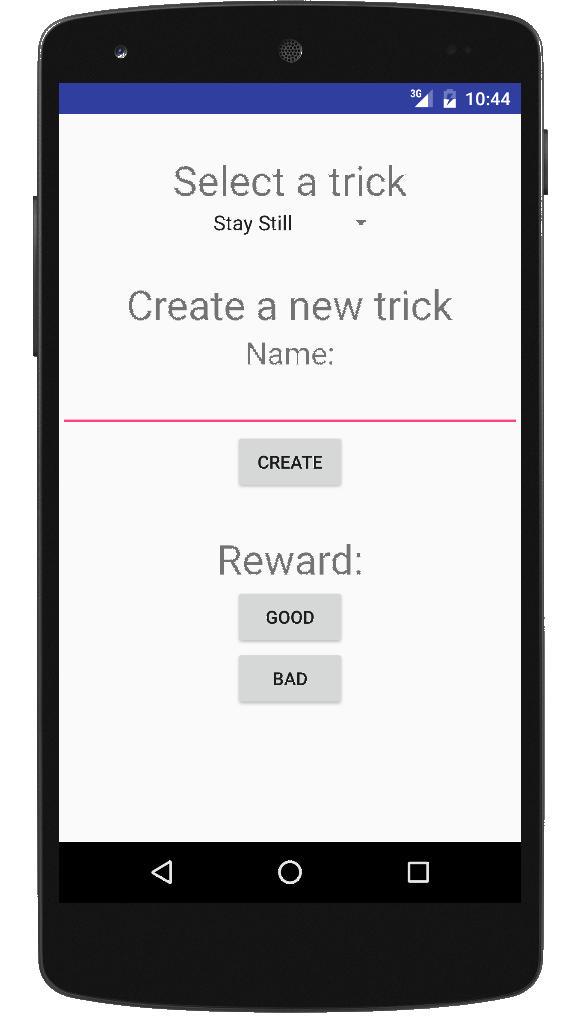
\includegraphics[height=7cm]{Figures/AppShot.png}
	\caption{Android Training Application Screenshot}
\end{figure}

Data was next collected from Fido's hardware implementation to gage performance with human given feedback in real world situations.
 Tasks were configured through the Android application previously discussed, allowing easy setting of hyper parameters such as neural network structure.
 The Android application also allowed for a more direct form of administering positive and negative reinforcement.


\subsubsection{Physical Experiments}

The first task given to Fido's hardware implementation was ``Stay Still,'' and as the name suggests Fido's sole responsibility for this task was to not move.
Fido's feed-forward neural network had 3 hidden layers each with 10 neurons and outputted 3 wires to the wire-fitted interpolator.
The exploration constant in equation \ref{equ::boltzmann} was held at $0.5$.
Fido was then given a reward value equal to $1 - 2|m|$ where $m$ was the speed of Fido's motors ranging from -1 to 1.

Fido's hardware implementation tested on one more task, ``Drive to Point.'' As on the simulator, Fido was tasked with moving to a point by controlling a differential drive system.
  At the start of each trial, Fido and the point were placed randomly on a smooth, hardwood surface within 0.75 meters of one another.
Fido was told the ratio of its $x$ displacement to its $y$ displacement from its target point as well as its rotation.
Every fourth action that Fido made was chosen as a reward iteration, and Fido was given a reward value corresponding to its last action.
This reward value was chosen by the tester based on whether Fido moved toward the point or not.
Fido completed each trial when it was within 10 cm of the point.
Fido's feed-forward neural network had 4 hidden layers each with 10 neurons and outputted 5 wires to the wire-fitted interpolator.
The exploration constant in equation \ref{equ::boltzmann} was held at 0.2.

\subsubsection{Physical Findings}

25 trials were done for each task to gather the data shown in Table \ref{tab:data2}.
 As with the simulation, reward iterations values shown are the medians of the data collected while time data shown is the mean of the data collected.

\begin{table}[ht]
	\centering
	\begin{tabular}{@{}lccc@{}}
		\toprule
		Task             & Learning Iterations & Action Selection (ms) & Training Time (ms) \\ \midrule
		Stay Still       & 3                   & 1                    & 43.5                  \\
		Drive to Point   & 18                  & 4                     & 65                  \\
	\end{tabular}
	\caption{Number of Learning Iterations, Action Selection Time, and Training Time Per Iteration for Fido Hardware Tasks}
	\label{tab:data2}
\end{table}

Performance was slower on the hardware implementation than in simulation due to the limited computation power of the Intel Edison compute model compared to modern desktop computers.
 However, the results still demonstrated Fido's real world applicability through its ability to perform outside of a simulation environment.